\chapter{Avaliação}
\label{cap:avaliacao}

Antes de se utilizar um novo sistema, é conveniente proceder-se a testes alargados de verificação, para que se tome conhecimento do seu correcto funcionamento e das sobrecargas introduzidas, para que de modo possa ser utilizado como uma mais–valia.
O mecanismo implementado (\textit{MRoP}) foi avaliado funcionalmente através de diversos testes relativamente aos dados de entrada nos diversos componentes que o constituem.
Como existem diversas fontes de dados, administrador para controlar a monitorização, o processo a ser monitorizado, estruturas de dados do núcleo, etc, foram criados vários testes de modo a que todas estas fontes de dados sejam analisadas.
Para além destas fontes directas de dados foi, também testada a correcção de que todos os fluxos de dados obtidos, através da monitorização de rede, são exclusivos ao processo alvo.
Assim todos estes testes e avaliações foram executados com sucesso e serão apresentados na secção \ref{sec:eval_functional}.

Como um dos principais objectivos desta dissertação é criar um mecanismo com melhor desempenho que os anteriores, apresentados na secção \ref{sect:outras_abordagens}, foi assim necessário verificar se este tinha sido atingido.
Desta forma foi necessário efectuar testes de desempenho sobre \textit{MRoP}, de modo a verificar se este objectivo tinha sido atingido.
Os testes de desempenho estão apresentados na secção \ref{sec:eval_performance}, incidindo sobre o desempenho global na transferência de 1GB de dados, através de protocolos conhecidos, bem como através de testes de desempenho que visam o mecanismo de instrumentação e a estrutura de dados escolhida para manter o estado do processo alvo.

Por último serão apresentadas algumas conclusões sobre as análises efectuadas ao \textit{MRoP} na secção \ref{sec:five_chap_conclusion}.

\section{Avaliação Funcional}
\label{sec:eval_functional}

A análise funcional ao \textit{MRoP} teve várias vertentes, uma vez que este mecanismo recebe dados de diferentes fontes, assim os testes visaram a verificação dos dados indicados pelo administrador, pelo processo alvo, e os das estruturas do núcleo.
Foi necessário garantir que não existiam falhas nos mecanismo de entrada de dados ao \textit{MRoP}, porque uma vez que este está a executar no núcleo tem acesso a todo o sistema, assim qualquer problema na validação de dados poderia comprometer o sistema a tanto nível de segurança como a nível de disponibilidade.



\subsection{Teste ao componente de controlo}

Como o \textit{MRoP} foi desenvolvido para ser um módulo para o núcleo, é necessário que seja adicionado a este através do programa \textit{insmod} ou semelhante.
Após a adição do \textit{MRoP} ao núcleo, para funcionar é necessário ser um utilizador com permissões de administrador (\textit{root}), e escrever em determinados ficheiros criados no \textit{DebugFs} para o controlo do \textit{MRoP}.
Dado que o \textit{MRoP} é parte do núcleo, é necessário garantir que qualquer dado que lhe é passado não compromete a segurança nem a disponibildade do sistema, por isso as funções que recebem dados oriundos do sistema de controlo efectuam verificações antes de os passar para as restantes componentes do \textit{MRoP}.
Como os dados de controlo são cadeias de caracteres, a função de verificação limita o tamanho máximo de caracteres, baseado no valor máximo expectável para a utilização do ficheiro.
Assim cadeias de caracteres maiores que um certo tamanho são truncadas, não existindo a possibilidade de explorar falhas de "\textit{under}" ou "\textit{overflow}", pois os valores inteiros são declarados sem sinal.
O valor zero (\textit{0}) serviu como valor inicializador, sendo que valores superiores a este, indicadores de que existe uma opção activa no \textit{MRoP}.
Para além destas análise, foram também verificadas que as permissões dos ficheiros estão de acordo com o estritamente necessário, e que apenas estão disponíveis ao utilizador \textit{root}.

\subsection{Obtenção do estado dos canais do processo alvo}

A análise funcional de detecção dos protocolos, portos e endereços locais, foi efectuada recorrendo à criação de dois conjuntos de programas \textit{cliente/servidor}.
Para o primeiro conjunto foi criado um servidor e um cliente, ambos utilizando o protocolo \textit{tcp}, em que o programa servidor esperava conexões numa porta e endereço pré-definidos.
Como o \textit{MRoP} instrumenta as chamadas ao sistema \textit{connect}, \textit{accept}, \textit{bind}, \textit{recvfrom}, \textit{sendto} e a função \textit{sock\_close}, é possível capturar todas as operações relativamente às comunicações de rede utilizando os protocolos \textit{tcp} e \textit{udp}.
Nas chamadas ao sistema \textit{bind} e \textit{connect}, um dos seus argumentos é uma estrutura \textit{sockaddr} que contém informações sobre o endereço e porto, sendo que na função \textit{connect} estes são relativos ao destino, e na função \textit{bind} são relativos à origem.
Num \textit{socket} recentemente criado, as estruturas \textit{socket} e \textit{sock} que lhe pertencem no núcleo, ainda não contém os dados relativos aos portos e endereços, assim os dados anteriormente mencionados são de extrema utilidade para a construção do repositório do \textit{MRoP}, de modo a capturar apenas o tráfego respeitante ao processo alvo.
Como os dados são provenientes do processo alvo, não é possível confiar que estão correctos, assim caso a função a executar retorne com um valor de erro, os valores adicionados são retirados do repositório, ficando novamente num estado consistente com a realidade.
De modo a verificar que os dados que se encontram no repositório estão completos e correctos, é efectuada a leitura de todos os valores do repositório e apresentados através da função \textit{printk} para o terminal do núcleo, ou então são apresentados no ficheiro criado para o efeito no sistema de ficheiros virtual \textit{DebugFs}, verificando se são os mesmo que a aplicação \textit{netstat} declara para o processo alvo.

Quando o processo alvo já se encontra em execução e se inicia a monitorização, os dados relativos aos protocolos, portos e endereços dos \textit{sockets}, estão presentes nas estruturas do núcleo, e por isso consideram-se correctos e válidos, caso tenham sido inicializados, sendo automaticamente adicionados ao repositório.



\subsection{Avaliação das estruturas dos \textit{sockets} no núcleo}

Os testes no núcleo utilizaram a função \textit{printk} para mostrar as informações necessárias no registo do núcleo, que pode ser acedido em nível utilizador através do programa \textit{dmesg} ou directamente do ficheiro \textit{messages} no directório $\backslash$\textit{var}$\backslash$\textit{log}.

Foram criados dois sistema simples de cliente/servidor, um utilizando canais \textit{tcp} e o outro canais \textit{udp}, de modo a verificar como os diferentes \textit{sockets} representam os dados referentes aos portos, endereços e protocolos no núcleo.
Os servidores esperavam conecções numa porta escolhida previamente, permitindo que os clientes efectuassem conecções para estes.
Nos servidores e nos clientes eram apresentados os endereços de memória da estrutura de dados (\textit{struct sockaddr}), que contém as propriedades dos \textit{sockets}, tais como, porto, endereço, protocolo, etc.

A utilização de \textit{KRetProbes} permitiu que se garantisse a correcção dos dados, uma vez que se os dados que não estivessem de acordo com o esperado, o núcleo através do valor de retorno indicaria que existia algum problema.
Estas situações estão contempladas dado que na função de \textit{handler} de retorno, um dos primeiros dados a verificar é o valor de retorno indicado pela função instrumentada, caso este valor seja de erro, todas as alterações previamente introduzidas no repositório serão removidas, deixando assim o repositório consistente com o núcleo.

\subsection{Avaliação de monitorização de rede}

Foi efectuada uma avaliação da correcção dos dados transferidos entre dois processos, um cliente e outro servidor.
Estes testes apenas foram efectuados para protocolos assentes sobre \textit{tcp}, pois nestes temos a certeza que devido ao sistema de controlo de comunicação não existem falhas, permitindo assim analisar a transferência desde o seu início até ao seu término.
Assim a execução do teste consistiu na transferência de um ficheiro entre duas máquinas, ligadas por um \textit{switch} com portas a 100 \textit{Mbit/s}, através do protocolo aplicacional \textit{ftp}, enquanto existiam outros fluxos de rede de outros processos.
Foi escolhido este protocolo pois apesar de ser necessário conhecer \textit{à prior} a porta de comunicação com o servidor, a transmissão de dados é efectuada em outra porta negociada dinamicamente, permitindo assim demonstrar também o potêncial do \textit{MRoP}.
Todas as comunicações remotas referentes a esta transferência foram monitorizadas através do programa \textit{tcpdump}, com o módulo do núcleo \textit{MRoP} activo e com a indicação do processo a monitorizar.
Esta monitorização foi guardada através do \textit{tcpdump} num ficheiro para posterior análise através do \textit{Wireshark}.
Utilizando o ficheiro capturado no \textit{Wireshark}, foi possível observar que apenas os fluxos de rede da transferência existiam no ficheiro.
Após esta verificação, foi efectuada a recuperação do ficheiro transmitido através da agregação dos dados presentes nos pacotes, exceptuando os cabeçalhos.
Esta recuperação foi guardada num ficheiro temporário, de modo a poderem ser aplicadas funções de sintese (\textit{md5} e \textit{sha1}), a fim de verificar que o conteúdo dos pacotes recuperado era exactamente igual ao ficheiro original, e à sua transferência.
Esta verificação foi confirmada através do mesmo valor retornado para os três ficheiros, para cada uma das funções de síntese utilizadas.

Como era necessário verificar também a correcção de transferências sobre o protocolo \textit{udp}, realizou-se um teste utilizado o programa \textit{iperf} com recurso a \textit{sockets} \textit{udp}.
Para a realização deste teste foi utilizada a mesma infra-estrutura de rede, em que numa das máquinas foi executado o \textit{iperf} em modo servidor utilizando \textit{sockets udp}, e na outra máquina foi executado o modo cliente também utilizando \textit{sockets udp}.
Foi efectuada a monitorização de rede na máquina que executou o \textit{iperf} em modo cliente, através do programa \textit{tcpdump} com o módulo do núcleo activo e com a indicação do identificador do processo \textit{iperf}, enquanto existiam outros fluxos de rede de outros processos.
O resultado da monitorização pelo \textit{tcpdump} foi guardado num ficheiro, que indicou que o total de \textit{bytes} correctamente recebidos pelo \textit{iperf} em modo servidor, foram também obtidos pela monitorização.
Neste ficheiro não existiam mais fluxos de dados que não os respeitantes à utilização do \textit{iperf}.

Como anteriormente referido, aquando dos testes existiram outros fluxos de rede, nomeadamente tráfego \textit{web}, de aplicações de conversação instantânea, entre outros, de modo a comprovar a eficácia de filtragem por processo.

\section{Avaliação do desempenho}
\label{sec:eval_performance}

Tendo presente a avaliação do desempenho, foram efectuados diversos testes com o objectivo de avaliar a sobrecarga gerada pela introdução do \textit{MRoP}.
Estes testes basearam-se na recepção ou transmissão de \textit{1 GigaByte} de dados, utilizando diferentes programas e protocolos, entre duas máquinas ligadas directamente.
Ambas as máquinas, que se optou por designar de máquina 1 e máquina 2, procederam à transmissão/recepção de dados, utilizando cada uma, apenas, um processador activo de 2 e de 2.6 Ghz, respectivamente.
As máquinas anteriormente descritas encontravam-se conectadas directamente, por interfaces de rede a 100 MBit/s, ficando uma das máquinas responsável pela execução dos servidores \textit{ftp}, \textit{http} e \textit{iperf}, e a outra pelos respectivos clientes.
A versão do sistema de operação utilizado, em ambas as máquinas, correspondeu ao 2.6.39, sendo que na máquina 1 foram introduzidas as modificações, para incluir o \textit{hook} do \textit{MRoP} e as suas funções auxiliares, enquanto na máquina 2 se executou o sistema original.

\subsection{Desempenho do \textit{MRoP}}


Na execução destes testes, foram efectuadas dez iterações, isto é, cada teste foi executado dez vezes, para cada experiência considerada, de modo a obter um valor médio e um desvio padrão considerado aceitável.
Os testes efectuados, em particular os primeiros, ilustram situações em que não há grande vantagem em ter o sistema o \textit{MRoP} activo, com vista a medir a sobrecarga do \textit{MRoP}.
Os resultados obtidos constam nas tabelas \ref{tab:desempenho} e \ref{tab:overhead}:

\begin{table}[!htb]
\begin{center}
\caption{Tempos médios em segundos (s)}
\begin{tabular}{ | c | c | c | c |  }
\hline
Teste & \hspace {0.3cm} Original \hspace {0.3cm}& \hspace {0.2cm} Com TcpDump \hspace {0.2cm} & Com TcpDump e MRoP \\
\hline
1GB - FTP$^{1}$ & 91.8508	& 91.8500 & 91.8854 \\
1GB - HTTP$^{2}$ & 91.6391 & 91.6472 & 91.6674 \\ 
IPerf - 1GB TCP$^{3}$ & 91.3790	& 91.2535	& 91.2672 \\
IPerf - 1GB UDP$^{4}$ & 89.7975 & 89.8007 & 89.8464 \\
\hline
\hline
1GB HTTP - 2 conexões$^{5}$ & 182.1573 & 188.7156 & 182.0161 \\
IPerf - 1GB UDP 2 conexões$^{6}$ & 179.4930 & 179.6280 & 179.6369 \\
\hline
\end{tabular}
\label{tab:desempenho}
\end{center}
\end{table}

\begin{table}[!htb]
\begin{center}
\caption{Sobrecarga das transferências (valores em percentagem)}
\begin{tabular}{ | c | c | c |}
\hline
Teste & \hspace {0.3cm} TcpDump \hspace {0.3cm} & TcpDump com MRoP  \\

\hline
1GB - FTP$^{1}$ & -0.0009  & 0.0377  \\
1GB - HTTP$^{2}$ & 0.0088 &  0.0309   \\
IPerf - 1GB TCP$^{3}$ & -0.1373 &  -0.1223   \\
IPerf - 1GB UDP$^{4}$ & 0.0036 & 0.0545 \\
\hline
\hline
1GB HTTP - 2 conexões$^{5}$ & 3.6003 & -0.0775   \\
IPerf - 1GB UDP 2 conexões$^{6}$ & 0.0752 & 0.0802   \\
\hline
\end{tabular}
\label{tab:overhead}
\end{center}
\end{table}

\begin{figure}[!ht]
\centering
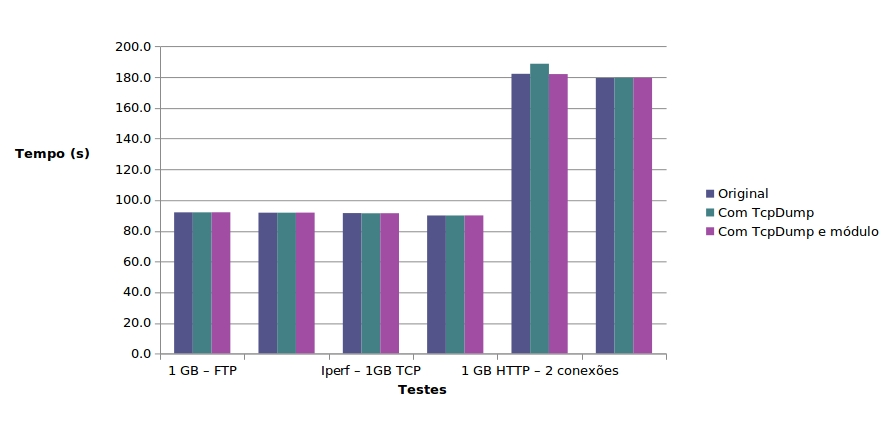
\includegraphics[scale=0.6]{testes.jpg}
\caption{Testes de desempenho efectuados ao MRoP}
\label{fig:tests_graphics}
\end{figure}

\begin{figure}[!ht]
\centering
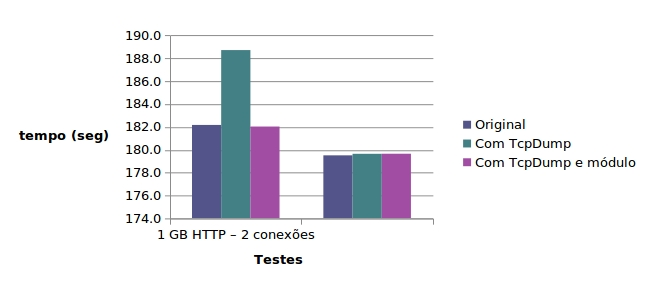
\includegraphics[scale=0.7]{overhead.jpg}
\caption{Sobrecarga nos testes 5 e 6 }
\label{fig:tests_overhead}
\end{figure}

Os primeiros quatro testes foram efectuados utilizando apenas uma conexão ao servidor, enquanto o 5º e o 6º testes utilizaram mais uma comunicação, de modo a aumentar o peso sobre o processador e o número de pacotes a circular entre as máquinas.
Desta forma, foi possível identificar a sobrecarga exercida enquando o \textit{tcpdump} executava e capturava todos os pacotes ou apenas um subconjunto destes, ou seja, os pacotes relativos aos processos alvo no novo sistema.
A coluna "Original" corresponde aos valores resultantes dos tempos médios das execuções das transferências na ausência de monitorização.
A coluna "Com \textit{TcpDump}" apresenta a média dos tempos de transferência com a captura total do tráfego utilizando a \textit{LibPCap}/\textit{LSF} original, enquanto que a coluna identificada com "Com \textit{TcpDump} e \textit{MRoP}" regista a média dos tempos para a transferência com captura pelo tcpdump e o módulo \textit{MRoP} desenvolvido no núcleo, de forma a capturar, apenas, o tráfego da transferência do processo alvo.
Nos primeiros quatro testes é possível verificar que a utilização do \textit{MRoP}, aumentou de forma insignificativa o tempo de execução (figura \ref{fig:tests_graphics}).
É igualmente possível observar que no 1º e 3º testes, aquando da utilização do \textit{tcpdump}, a execução sem o \textit{MRoP}, mostrou-se muito ligeiramente mais rápida, como se pode verificar na tabela \ref{tab:desempenho} e \ref{tab:overhead}.


Esta situação pode dever-se / deve-se ao facto de, quando a máquina se encontra em sobrecarga, leva ao aumento do tamanho médio dos pacotes, reduzindo o seu número e o volume de dados transferidos, em virtude da diminuição dos seus cabeçalhos.

Nos testes 5º e 6º testes, como o tráfego na interface é duplicado e o \textit{tcpdump} tem que capturar todos os pacotes, é possível evidenciar a sobrecarga exercida por estas cópias de dados e consequentes transferências (para nível utilizador) face ao novo sistema onde apenas captura um fluxo de dados.
Na tabela \ref{tab:overhead} e na figura \ref{fig:tests_overhead} é possível observar que, para o teste 5, a sobrecarga do \textit{tcpdump} atinge os 3.6\% face ao original, enquanto que a sobrecarga do \textit{tcpdump} com o \textit{MRoP}, permitiu uma ligeira melhoria face ao original (-0.0775\%).
Conclui-se, portanto, que quando o fluxo de dados que não pretendemos capturar aumenta consideravelmente, torna-se mais vantajoso utilizar o \textit{MRoP}, do que capturar todos os pacotes, na medida em que minimiza-se a sobrecarga, capturando apenas os dados relevantes, evitando-se assim a identificação e filtragem dos pacotes pertencentes ao processo alvo em nível utilizador (o que acarretaria uma sobrecarga adicional).

---------------------------

Comentar em relação ao efectuado por farruca 10 onde o overhead era cerca de 2\% 

----------------------------

\subsection{Desempenho da estrutura de dados}

Para além das avaliações anteriormente descritas, tornou-se essencial analisar o comportamento da estrutura de dados utilizado no componente “estado do processo”, de modo a verificar o seu desempenho.
Assim para esta análise, foi elaborado um teste para determinar o desempenho da estrutura de dados, em relação às inserções e remoções.
Este teste utiliza o sistema de alta resolução de temporizadores (\textit{HRTimer})\cite{hrtimerKernel}, presente no núcleo do sistema de operação.

O teste consistiu em obter o tempo anterior e posterior à inserção dos 1024 elementos, representando outros tantos portos/endereços, afim de determinar o tempo decorrido.
De igual modo, foi calculado o tempo de remoção dos referidos elementos.
Os resultados obtidos estão reproduzidos na tabela \ref{tab:tree_info}.


----------------------------------------------------------------------------------------------------------

A análise de desempenho da estrutura de dados

O número de elementos foi 1024, pois este valor foi obtido através da chamada ao sistema ------ que indica qual o máximo de canais que podem estar a ser utilizados por um processo.
Como os canais podem ser ficheiros, \textit{pipes}, \textit{sockets}, etc, o valor de uma utilização real deverá ser inferior a este, por isso considerou-se o valor de 1024 como um bom indicador do número de elementos que estrutura de dados, poderá conter num dado momento, permitindo assim verificar o desempenho desta com elevada carga.

A inserção de dados no repositório, não é efectuada com um desempenho constante, dado que quando é necessário efectuar um rebalanceamento da árvore, o processo de inserção é mais demorado devido à necessidade de efectuar rotações na árvore.

Os testes foram efectuados de modo a obtermos valores nos piores casos.

----------------------------------------------------------------------------------------------------------
 
\begin{table}[!htb]
\begin{center}
\caption{Custo das operações (tempos em nanosegundos)}
\begin{tabular}{ | r | c | c | }
\hline
\hspace{1cm} Teste \hspace{1.5cm} & \hspace{1cm}Duração\hspace{1cm} &  Média por
elemento \\
\hline
Adição de 1024 elementos & 869 244 & 848.8711 \\
\hline
Remoção de 1024 elementos & 675 086 & 659.2637\\
\hline

\hline
\end{tabular}
\label{tab:tree_info}
\end{center}
\end{table}

Como se pode verificar, pela tabela \ref{tab:tree_info}, a inserção de um elemento na árvore é inferior a 1 microsegundo, demonstrando que a estrutura utilizada não introduz uma elevada sobrecarga.
Para além de estabelecer um bom compromisso de desempenho e utilização de memória, a sua disponibilidade de utilização no núcleo do sistema, possibilitou ter um elevado grau de confiança na sua utilização.
O tempo médio despendido na procura do elemento com o menor valor de chave, nos 1024 elementos adicionados, foi de 1327 nanosegundos.
Com este valor é possível verificar que para efectuar 10 iterações de procura na árvore, incorre-se numa penalização de 1.3 microsegundos.
Verifica-se assim, que o tempo médio de procura de elementos na estrutura, é menor ou igual a 1.3 microsegundos.
Considerando que a maioria das aplicações não utiliza tantos portos em simultâneo, são expectáveis tempos inferiores em aplicações reais.


\subsection{Desempenho do Sistema de instrumentação}
Sendo a instrumentação das chamadas ao sistema um ponto fundamental na execução da monitorização de uma aplicação, a análise ao seu comportamento é bastante importante, na medida em que é necessário verificar se a introdução deste tipo de sistema irá produzir uma elevada penalização sobre o sistema de operação.
A análise efectuada consistiu em colocar um \textit{KRetProbe} na chamada ao sistema \textit{getpid} e avaliar o tempo decorrido entre o início e o fim do total das chamadas, com e sem o \textit{KRetProbe}, de forma a avaliar a sobrecarga e verificar se coincide com o indicado pelos criadores do sistema.
A chamada ao sistema escolhida foi o \textit{getpid}, pois esta é uma função muito simples que apenas devolve o identificador do processo que a invocou.

\providecommand{\e}[1]{\ensuremath{\times 10^{#1}}}

\begin{table}[!htb]
\begin{center}
\caption{Duração das chamadas em segundos}
\begin{tabular}{ | c | c | c | c |}
\hline
Teste & Original & Com \textit{KRetProbe} & Sobrecarga por chamada\\
\hline
100 000 000 chamadas & 12.65 &  73.6600 & 610.10\e{-9}\\
1 000 000 000 chamadas & 126.85 & 737.2100 & 610.36\e{-9}\\
\hline
\end{tabular}
\label{tab:kprobes_info}
\end{center}
\end{table}

O valor de referência obtido pelos criadores do \textit{KProbes}, referentes ao \textit{KRetProbe} sem optimizações, é de 0.7 microsegundos\cite{KProbeKernel}, sendo que o valor médio obtido foi de 0.61 microsegundos, ou seja, ligeiramente inferior, visto que a máquina de referência apresenta uma frequência de \textit{cpu} inferior à máquina onde foram realizados estes testes.

Consideram-se estes valores bastante aceitáveis e espera-se que tenham ainda reduzido impacto no desempenho normal do sistema.
Note-se ainda que esta instrumentação só é introduzida aquando do carregamento do módulo para executar a monitorização com esta nova funcionalidade.

\section{Conclusão}
\label{sec:five_chap_conclusion}

Com os testes efectuados ao nível funcional e ao nível de desempenho ao \textit{MRoP} verificou-se que este mecanismo oferece um desempenho aceitável nas condições mais adversas, o que indica que para as condições das aplicações reais o seu desempenho será superior, enquanto que a sobrecarga introduzida no sistema poderá ser inferior ao constatado.

Como se pode verificar em relação ao trabalho \cite{}, a sobrecarga gerada pelo \textit{MRoP} foi muito inferior, o que demonstra que apesar da dificuldade de trabalhar no núcleo, evitar situações de análise em nível utilizador foi largamente compensado pelo trabalho efectuado no núcleo.

